\documentclass[a4paper,11pt]{article}
\usepackage{fullpage}
\usepackage[latin1]{inputenc}
\usepackage[T1]{fontenc}
\usepackage[normalem]{ulem}
\usepackage[english]{babel}
\usepackage{listings,babel}
\lstset{breaklines=true,basicstyle=\ttfamily}
\usepackage{graphicx}
\usepackage{moreverb}
\usepackage{url}

\title{Implementing MilkDrop on Milkymist}
\author{S\'ebastien Bourdeauducq}
\date{\today}
\begin{document}
\setlength{\parindent}{0pt}
\setlength{\parskip}{5pt}
\maketitle{}
\section{Introduction}
MilkDrop is a popular, hardware-accelerated music visualization plugin for Winamp. MilkDrop is an environment for running presets, software which controls MilkDrop, and does not produce visualizations by itself.

Presets are saved in .milk format. Creating new presets is generally referred to as authoring, or writing, making the person that wrote a preset its author. Presets are distributed on the internet though Winamp, the Winamp Forums, and through the personal webpages of MilkDrop preset authors. A preset's title also doubles as its .milk save name, and usually includes the preset author or authors' pseudonym.

This document explains how to render such presets, with a focus on implementing them in Milkymist.

\section{Overview}
A \verb!.milk! file is composed of 2 major different kinds of scriptable equations. These are per\_frame and per\_vertex (sometimes called per\_pixel) equations.

Code in the per\_frame section is done once for each frame, modifying variables which affect different parameters that can be passed to other areas of code. Trigonometric functions which modify MilkDrop's internal looping time variable, systems of logic, and interaction with the audio information can be used to govern how these parameters evolve though time.

The screen is divided into a grid and the per\_vertex code is evaluated at each grid point (vertex). The pixels in-between these points interpolate their values from the surrounding 4 points on the grid. The size of the grid is 32x24 by default, but can be set higher or lower by the user. Per\_vertex equations allow the preset author to alter some of MilkDrop's parameters differently in certain areas of the screen based upon x and y values, distance from the center of the screen, and the angle.

More information is available in preset authoring guides available from MilkDrop website.

A diagram of the operations for rendering a preset is shown in Figure~\ref{fig:flow}.
\begin{figure}[htp]
\centering
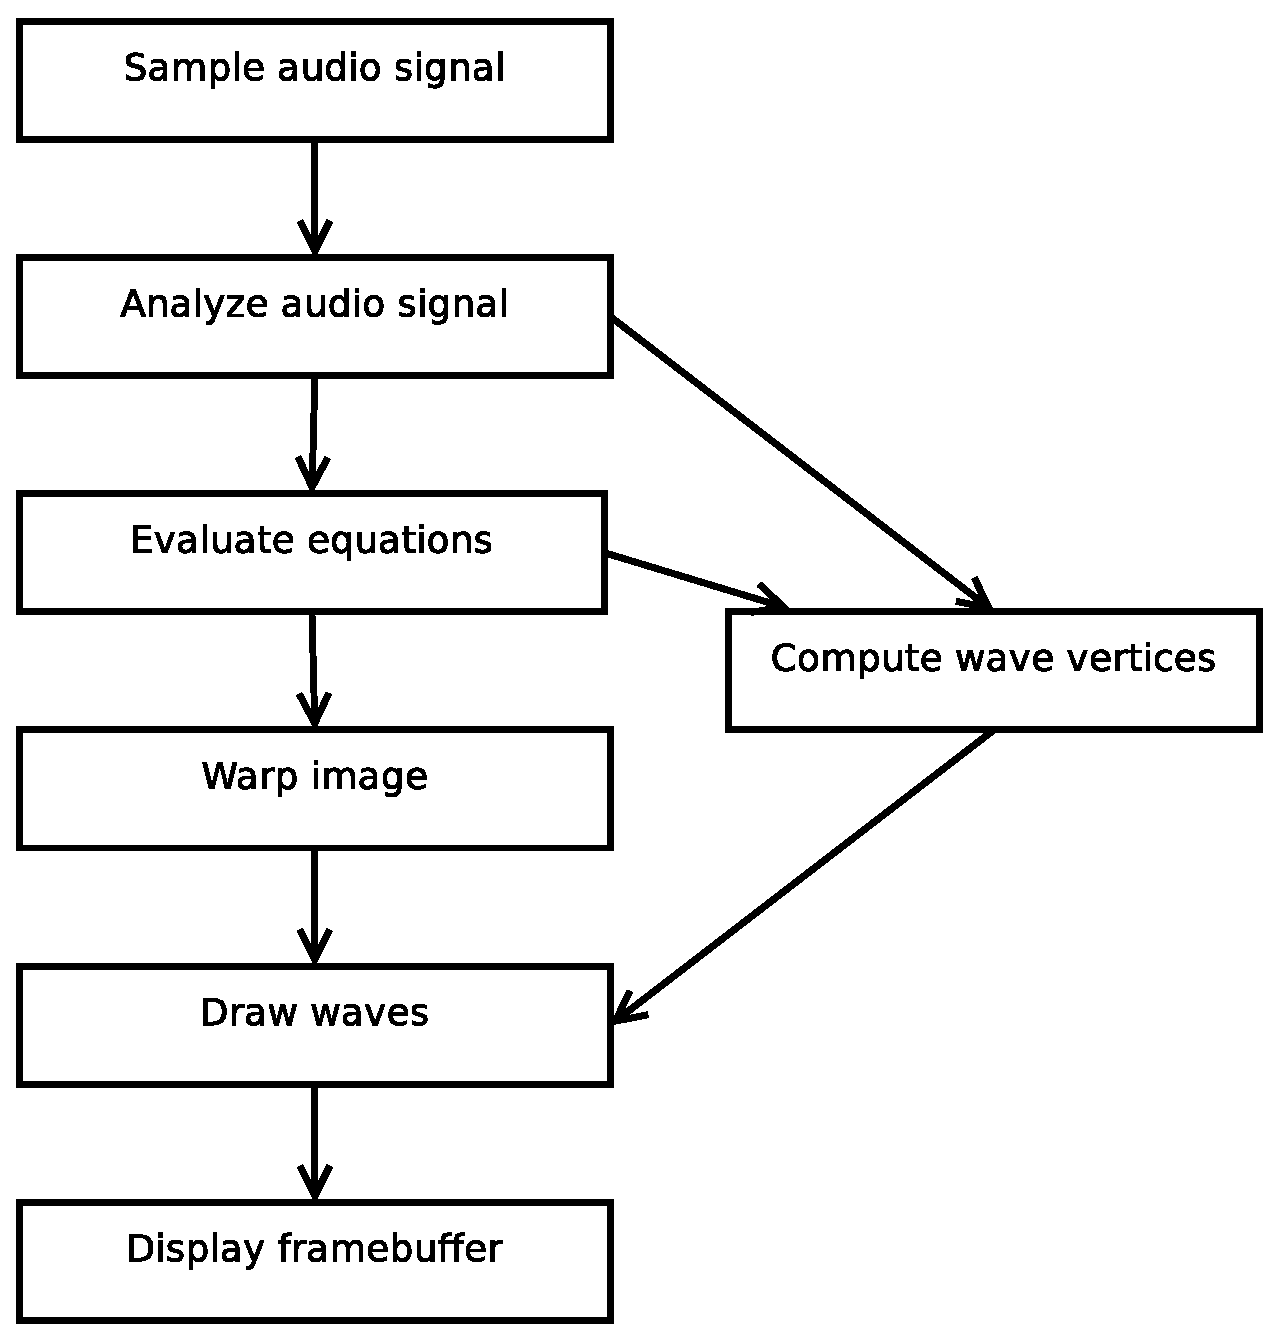
\includegraphics[height=80mm]{flow.eps}
\caption{The rendering flow.}\label{fig:flow}
\end{figure}

\section{Generating the warping mesh}
In a MilkDrop preset, the warping mesh is computed from a set of parameters that can be fixed or generated by the per-frame and per-vertex equations.

Those parameters are the following:
\begin{itemize}
\item \verb!zoom!, which scales the image.
\item \verb!zoomexp!, which (locally) zooms the image more when getting further from the center.
\item \verb!sx!, \verb!sy!, \verb!cx! and \verb!cy!, which scales the image on X and Y axises around the point $ (cx, cy) $.
\item \verb!warp!, \verb!fWarpScale! and \verb!fWarpAnimSpeed!, which distort the image.
\item \verb!rot!, \verb!cx! and \verb!cy!, which rotates the image around the point $ (cx, cy) $.
\item \verb!dx! and \verb!dy!, which add a delta to the mesh point.
\end{itemize}

In the rendering process, every new frame is based on the old one warped using these parameters. For instance, this means that if the \verb!rot! parameter is held constant at a non-zero value, you get a continuous spiral movement, not a simple shift of the image.

Now, we need a formal description of what these parameters do.

In projectM 1.1 (an OpenGL implementation of MilkDrop), the warping is done via the method \verb!Renderer::Interpolation!, defined in \verb!Renderer.cpp!. This method just programs the GPU for doing image warping and decay. The warping mesh is passed in \verb!presetOutputs->x_mesh! and \verb!presetOutputs->y_mesh!, and the decay value in \verb!presetOutputs->decay!. The mesh coordinates are floating-point numbers between 0 and 1, which means the top-left corner of the screen is at $ (0, 0) $, the bottom-right at $ (1, 1) $ and the center at $ (0.5, 0.5) $.

The generation of the mesh is done from the per-frame and per-vertex equations results by the \verb!Renderer::PerPixelMath! method.

The order of the operations performed by this function is:
\begin{itemize}
\item make an initial zoomed mesh:
\[
\left\{ \begin{array}{rrlr}
zoom2(x, y) & = & zoom(x, y)^{zoomexp(x, y)^{rad(x, y) \cdot 2 - 1}} \\
meshx(x, y) & = & ( idx(x, y) - 0.5) \cdot zoom2(x, y) + 0.5 \\
meshy(x, y) & = & ( idy(x, y) - 0.5) \cdot zoom2(x, y) + 0.5
\end{array}
\right.
\]
with $ x $ and $ y $ representing the indexes of the current mesh point, $ zoom $ and $ zoomexp $ the results of the per-vertex equations, $ rad $ the distance from the center of the screen and $ idx $ and $idy $ the mesh for which no image transformation is performed (the image is copied verbatim), defined by:
\[
\left\{ \begin{array}{rrlr}
idx(x, y) & = & \frac{x}{meshcountx-1} \\
idy(x, y) & = & \frac{y}{meshcounty-1}
\end{array}
\right.
\]

For most presets, $ zoomexp = 1 $, so in the first versions of Milkymist we could use $ zoom2(x, y) = zoom(x, y) $.

\item scale the mesh according to \verb!sx! and \verb!sy!:
\[
\left\{ \begin{array}{rrlr}
meshx(x, y) & = & \frac{meshx(x, y) - cx(x, y)}{sx(x, y)} + cx(x, y)\\
meshy(x, y) & = & \frac{meshy(x, y) - cy(x, y)}{sy(x, y)} + cy(x, y)
\end{array}
\right.
\]

\item apply the effect triggered by the \verb!warp! parameter, using those magic formulas:
\[
\left\{ \begin{array}{rrlr}
wt & = & time \cdot animspeed \\
s & = & \frac{1}{scale} \\
f_0 & = & 23.36 + 8 \cdot cos(wt \cdot 1.413 + 10) \\
f_1 & = & 17.54 + 6 \cdot cos(wt \cdot 1.113 + 7) \\
f_2 & = & 21.08 + 6 \cdot cos(wt \cdot 1.233 + 3) \\
f_3 & = & 22.98 + 8 \cdot cos(wt \cdot 0.993 + 5) \\
meshx(x, y) & = & meshx(x, y) \\
 &  & + warp \cdot 0.0035 \cdot sin(wt \cdot 0.333 + s \cdot (idx(x, y) \cdot f_0 - idy(x, y) \cdot f_3)) \\
 &  & + warp \cdot 0.0035 \cdot cos(wt \cdot 0.753 - s \cdot (idx(x, y) \cdot f_1 - idy(x, y) \cdot f_2)) \\
meshy(x, y) & = & meshy(x, y) \\
 &  & + warp \cdot 0.0035 \cdot cos(wt \cdot 0.375 - s \cdot (idx(x, y) \cdot f_2 + idy(x, y) \cdot f_1)) \\
 &  & + warp \cdot 0.0035 \cdot sin(wt \cdot 0.825 + s \cdot (idx(x, y) \cdot f_0 + idy(x, y) \cdot f_3)) \\
\end{array}
\right.
\]

\item apply the rotation
\[
\left\{ \begin{array}{rrlr}
u(x, y) & = & meshx(x, y) - cx(x, y) \\
v(x, y) & = & meshy(x, y) - cy(x, y) \\
meshx(x, y) & = & u(x, y) \cdot cos(rot(x, y)) - v(x, y) \cdot sin(rot(x, y)) + cx(x, y) \\
meshy(x, y) & = & u(x, y) \cdot sin(rot(x, y)) + v(x, y) \cdot cos(rot(x, y)) + cy(x, y)
\end{array}
\right.
\]

\item apply the deltas
\[
\left\{ \begin{array}{rrlr}
meshx(x, y) & = & meshx(x, y) + dx(x, y)\\
meshy(x, y) & = & meshy(x, y) + dy(x, y)
\end{array}
\right.
\]

\end{itemize}

\section{Software architecture}
\begin{figure}[htp]
\centering
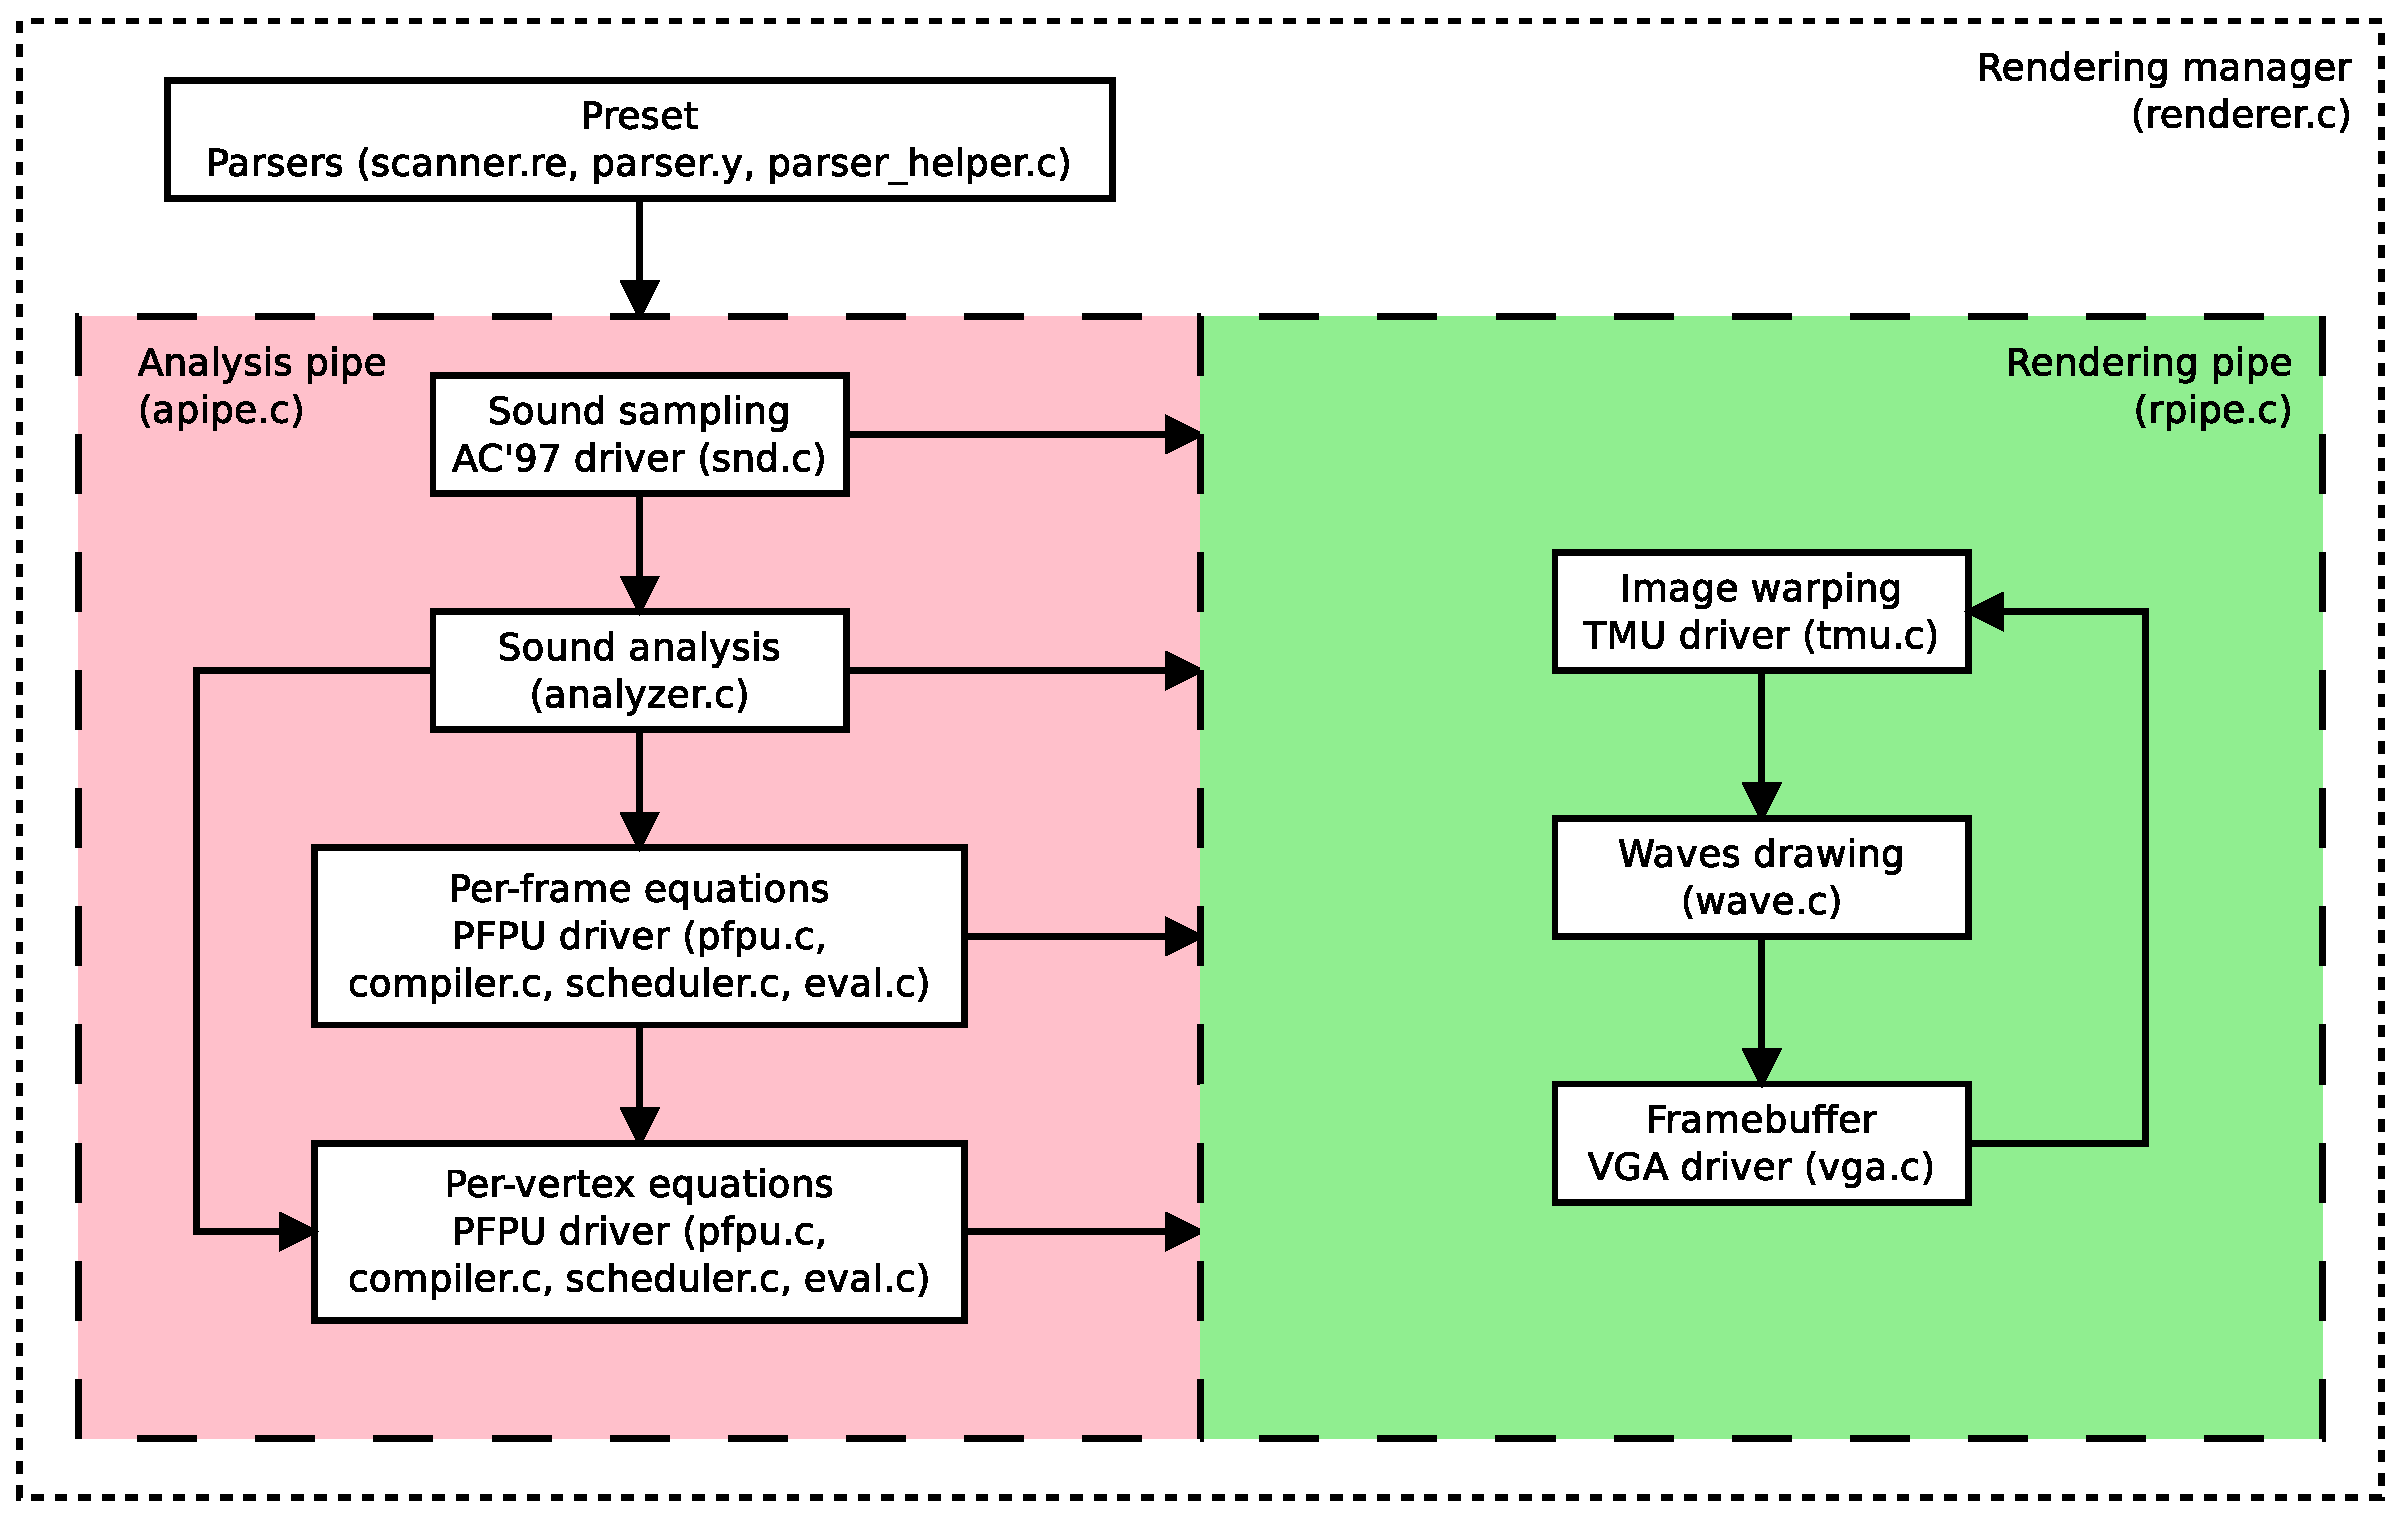
\includegraphics[height=90mm]{swarch.eps}
\caption{Software architecture of the rendering system.}\label{fig:swarch}
\end{figure}

\end{document}
